\documentclass[a4paper,12pt]{article}
\usepackage{url}
\usepackage{parskip} 	
\usepackage{tabularx}

%other packages for formatting
\RequirePackage{color}
\RequirePackage{graphicx}
\usepackage[usenames,dvipsnames]{xcolor}
\usepackage[scale=0.9]{geometry}
\usepackage{amsmath}
\usepackage{tikz}
\usetikzlibrary{shapes,arrows}
\usepackage{rotating}
\usetikzlibrary{shapes.geometric, arrows}
\usetikzlibrary{positioning, shapes}
\usepackage{float}
\usepackage{algorithm}
\usepackage{algpseudocode}
\usepackage{tikz}
\usetikzlibrary{arrows.meta, positioning}
\usepackage{setspace}
\usepackage{titlesec}
\usepackage{tikz}
\usepackage{tabularx}
\usepackage{circuitikz}
\usepackage{pgfplots}
\usepackage{amssymb}
\usepackage{amsthm}
\usepackage{float}  
\usepackage{booktabs}
\usepackage{xcolor}
\pgfplotsset{compat=1.18}
\usepackage{setspace}
\usepackage{colortbl}
\usepackage{tcolorbox}
\usepackage{wrapfig}
\usepackage{media9}
\usepackage{siunitx}

% Define colors
\definecolor{blueblock}{RGB}{173, 216, 230}  % Light blue
\definecolor{greenblock}{RGB}{144, 238, 144} % Light green
\definecolor{redblock}{RGB}{255, 182, 193}   % Light red
\definecolor{lightblue}{RGB}{173,216,230}
\definecolor{lightgreen}{RGB}{144,238,144}
\definecolor{lightorange}{RGB}{255,200,150}
\definecolor{lightpurple}{RGB}{220,180,240}

\tikzstyle{startstop} = [rectangle, rounded corners, minimum width=3cm, minimum height=1cm,text centered, draw=black, fill=red!30]
\tikzstyle{process} = [rectangle, minimum width=3cm, minimum height=1cm, text centered, draw=black, fill=blue!30]
\tikzstyle{decision} = [diamond, minimum width=3cm, minimum height=1cm, text centered, draw=black, fill=green!30]
\tikzstyle{arrow} = [thick,->,>=stealth]
\tikzstyle{io} = [trapezium, trapezium left angle=70, trapezium right angle=110, minimum width=3cm, minimum height=1cm, text centered, draw=black, fill=blue!30]

% Define styles with smaller dimensions and font size
\tikzset{
    font=\small,
    startstop/.style={
        rectangle,
        rounded corners,
        minimum width=2.5cm,
        minimum height=0.8cm,
        draw=black,
        fill=red!30,
        text centered,
        % Set text width to wrap text automatically
        text width=3.0cm,
        align=center
    },
    process/.style={
        rectangle,
        minimum width=2.5cm,
        minimum height=0.8cm,
        draw=black,
        fill=orange!30,
        text centered,
        % Set text width to wrap text automatically
        text width=3.0cm,
        align=center
    },
    decision/.style={
        diamond,
        aspect=2,
        draw=black,
        fill=green!30,
        inner sep=0pt,
        minimum width=2.0cm,
        minimum height=1.0cm,
        % Allow text wrapping in decision blocks
        text width=2.2cm,
        align=center
    },
    io/.style={
        trapezium,
        trapezium left angle=70,
        trapezium right angle=110,
        minimum width=2.5cm,
        minimum height=0.8cm,
        draw=black,
        fill=blue!30,
        text centered,
        % Set text width to wrap text automatically
        text width=3.0cm,
        align=center
    },
    arrow/.style={
        thick,
        ->,
        >=Stealth,
        shorten <=1pt,
        shorten >=1pt
    },
}

\definecolor{codegreen}{rgb}{0,0.6,0}
\definecolor{codegray}{rgb}{0.5,0.5,0.5}
\definecolor{codepurple}{rgb}{0.58,0,0.82}
\definecolor{backcolour}{rgb}{0.95,0.95,0.92}

\usepackage{listings}

% Define C style
\lstdefinestyle{cstyle}{
    backgroundcolor=\color{backcolour},
    commentstyle=\color{codegreen},
    keywordstyle=\color{blue}, % Keywords in blue
    numberstyle=\tiny\color{codegray},
    stringstyle=\color{codepurple},
    basicstyle=\ttfamily\footnotesize,
    breakatwhitespace=false,
    breaklines=true,
    captionpos=b,
    keepspaces=true,
    numbers=left,
    numbersep=5pt,
    showspaces=false,
    showstringspaces=false,
    showtabs=false,
    tabsize=4,
    language=C,
    morekeywords={uint32_t, uint64_t, int32_t, int64_t, bool, inline}
}

\lstset{style=cstyle}

% Page layout settings
\geometry{a4paper, margin=1in}

%tabularx environment
\usepackage{tabularx}

%for lists within experience section
\usepackage{enumitem}

% centered version of 'X' col. type
\newcolumntype{C}{>{\centering\arraybackslash}X} 

%to prevent spillover of tabular into next pages
\usepackage{supertabular}
\usepackage{tabularx}
\newlength{\fullcollw}
\setlength{\fullcollw}{0.47\textwidth}

%custom \section
\usepackage{titlesec}				
\usepackage{multicol}
\usepackage{multirow}

%CV Sections inspired by: 
%http://stefano.italians.nl/archives/26
\titleformat{\section}{\large\scshape\raggedright}{}{0em}{}[\titlerule]
\titlespacing{\section}{0pt}{10pt}{10pt}

%for publications
\usepackage[style=authoryear,sorting=ynt, maxbibnames=2]{biblatex}

%Setup hyperref package, and colours for links
\usepackage[unicode, draft=false]{hyperref}
\definecolor{linkcolour}{rgb}{0,0.2,0.6}
\hypersetup{colorlinks,breaklinks,urlcolor=linkcolour,linkcolor=linkcolour}
\addbibresource{citations.bib}
\setlength\bibitemsep{1em}

%for social icons
\usepackage{fontawesome5}
\graphicspath{{../Images/}}

\begin{document}
%----------------------------------------------------------------------------------------
%	TITLE+
%----------------------------------------------------------------------------------------
% Title Page
\begin{titlepage}
    \centering
    \vspace*{2cm}
    \Huge{\textbf{EEE3027 Integrated Circuit Design}}\\[0.5cm]
    \Large{\textbf{Semester 1 Report}}\\ 
    \Large{Sahas Talasila \textit{230057896}}
    \vfill
\end{titlepage}

% Table of Contents
\tableofcontents
\newpage

\begin{abstract}
    This is a placeholder for the abstract of the report.
\end{abstract}

\section{Introduction}

\subsection{Background and Key Concepts}

\subsubsection{Transistors}
A transistor is a semiconductor device used to amplify or switch electronic signals and electrical power. 
It is composed of semiconductor material, usually with at least three terminals for connection to an external circuit. A voltage or current applied to one pair of the transistor's terminals controls the current through another pair of terminals.

\textbf{Transistor Structure:}

\begin{itemize}
    \item \textbf{Source (S):} The terminal through which carriers enter the channel.
    \item \textbf{Drain (D):} The terminal through which carriers leave the channel.
    \item \textbf{Gate (G):} The terminal that modulates the conductivity of the channel.
    \item \textbf{Body (B):} The substrate on which the transistor is built, often connected to the source.
    \item \textbf{Channel:} The region between the source and drain where current flows when the transistor is on.  
    \item \textbf{Oxide Layer:} An insulating layer between the gate and the channel, typically made of silicon dioxide (SiO2).
\end{itemize}

\begin{figure}[h!]
    \centering
    \begin{circuitikz}[american]

  % NMOS transistor
  \draw
    (0,0) node[nmos, anchor=D] (nmos) {}
    (nmos.G) node[left] {G}
    (nmos.D) node[above] {D}
    (nmos.S) node[below] {S};

  % PMOS transistor with flipped orientation
  \draw
    (4,0) node[pmos, anchor=S, xscale=-1] (pmos) {}
    (pmos.G) node[right] {G}
    (pmos.D) node[below] {D}
    (pmos.S) node[above] {S};
\end{circuitikz}
    \caption{Basic structure of an NMOS and PMOS transistor.}
    \label{fig:transistor_structure}
\end{figure}

\subsubsection{MOSFET Types}
\begin{itemize}
    \item \textbf{N-channel (NMOS):} electrons are charge carriers.
    \item \textbf{P-channel (PMOS):} holes are charge carriers.
\end{itemize}

\subsubsection{Operating Regions of a MOSFET}
\begin{center}
\begin{tabular}{|c|c|c|}
\hline
\textbf{Region} & \textbf{Condition (N-channel)} & \textbf{Description} \\
\hline
Cutoff & $V_{GS} < V_{th}$ & OFF (no current) \\
Triode (Linear) & $V_{GS} > V_{th}, \, V_{DS} < V_{GS}-V_{th}$ & Acts as variable resistor \\
Saturation (Active) & $V_{GS} > V_{th}, \, V_{DS} \ge V_{GS}-V_{th}$ & Current source (amplifier region) \\
\hline
\end{tabular}
\end{center}

\subsection{Importance of MOSFET Physical Parameters}

The physical dimensions of a MOSFET determine its performance in terms of speed, power, and reliability.

\subsubsection{Key Parameters and Effects}
\begin{center}
\begin{tabular}{|c|c|c|}
\hline
\textbf{Parameter} & \textbf{Symbol} & \textbf{Importance} \\
\hline
Gate Length & $L$ & Controls speed/gain; shorter $L$, more speed but causes leakage. \\
Gate Width & $W$ & Controls current; wider $W$, more current and capacitance. \\
Oxide Thickness & $t_{ox}$ & Thinner ox - improves gate control but increases tunneling. \\
Channel Depth & -- & Affects channel formation and conductivity. \\
Threshold Voltage & $V_{th}$ & Determines switching voltage. \\
Junction Depth & -- & Impacts short-channel effects and capacitance. \\
\hline
\end{tabular}
\end{center}

\subsubsection{Significance}
\begin{itemize}
    \item \textbf{Speed:} shorter channel $\Rightarrow$ faster switching.
    \item \textbf{Power Efficiency:} optimized $V_{th}$ and $t_{ox}$ reduce power loss.
    \item \textbf{Current Drive:} larger $W$ gives more drive capability.
    \item \textbf{Reliability:} careful balance of parameters prevents breakdown and leakage.
\end{itemize}

\subsection{Gain}

\subsubsection{Definition}
\textbf{Gain} is the ratio of output signal to input signal, as shown by \textit{Equations 1 and 2}:
\begin{equation}
    \text{Gain} = \frac{\text{Output}}{\text{Input}}
\end{equation}

Types include:
\begin{equation}
A_v = \frac{V_{out}}{V_{in}}, \quad
A_i = \frac{I_{out}}{I_{in}}, \quad
A_p = \frac{P_{out}}{P_{in}}
\end{equation}

\subsubsection{Gain in BJTs and MOSFETs}

\textit{Equations 3 and 4} show gain definitions for BJTs and MOSFETs:

\begin{equation}
    \text{BJT current gain} \beta = \frac{I_C}{I_B}
\end{equation}

\begin{equation}
    \text{MOSFET transconductance} g_m = \frac{\partial I_D}{\partial V_{GS}} = \beta(V_{GS} - V_{th})
\end{equation}

\subsubsection{Gain in Decibels}
Gain in decibels (dB) is given by \textit{Equation 5}

\begin{equation}
\text{Voltage Gain (dB)} = 20 \log_{10}\left(\frac{V_{out}}{V_{in}}\right)    
\end{equation}:


\subsubsection{Importance}
\begin{itemize}
    \item Determines amplification strength.
    \item Critical in analogue amplifiers, control systems, and logic gates.
\end{itemize}

\subsection{Gate Length vs. Channel Length}

\begin{itemize}
    \item \textbf{Gate Length ($L_G$):} physical distance between source and drain under the gate.
    \item \textbf{Channel Length ($L_{CH}$):} effective electrical distance current travels.
\end{itemize}

They are related by \textit{Equation 6}:
\begin{equation}
L_{CH} = L_G - \Delta L    
\end{equation}

where $\Delta L$ is due to lateral diffusion of dopants.

\subsubsection{Difference and Importance}
Shorter effective channel length causes:
\begin{itemize}
    \item Increased leakage and short-channel effects.
    \item Lower threshold voltage.
    \item Reduced control by the gate.
\end{itemize}

%--------------------------------------------------------------
\subsection{Beta ($\beta$) Equations for MOSFETs}

Shown by \textit{Equations 7 and 8}:

\subsubsection{Definition}
\begin{equation}
I_D = \frac{1}{2}\beta(V_{GS} - V_{th})^2 \quad \text{(saturation region)}    
\end{equation}

\begin{equation}
I_D = \beta\left[(V_{GS} - V_{th})V_{DS} - \frac{V_{DS}^2}{2}\right] \quad \text{(linear region)}
\end{equation}

\subsubsection{Beta Expression}

Beta can also be expressed by \textit{Equation 9}:

\begin{equation}
\boxed{\beta = \mu_n C_{ox} \frac{W}{L}}
\end{equation}

where:
\begin{itemize}
    \item $\mu_n$ = carrier mobility
    \item $C_{ox} = \frac{\varepsilon_{ox}}{t_{ox}}$ = oxide capacitance per unit area
    \item $W$ = gate width
    \item $L$ = gate length
\end{itemize}

\subsubsection{Related Terms}
\[
k' = \mu_n C_{ox}, \quad \beta = k'\frac{W}{L}
\]
\[
g_m = \frac{\partial I_D}{\partial V_{GS}} = \beta(V_{GS} - V_{th})
\]

\subsubsection{Importance}
\begin{itemize}
    \item Determines how strongly a MOSFET amplifies a signal.
    \item Affects gain, speed, and current drive.
    \item Critical for matching and biasing in analogue ICs.
\end{itemize}

\section{Formative Assessment 1 Report}

A MOS transistor operates in two main regions depending on the drain-source voltage ($V_{DS}$) and the gate-source voltage ($V_{GS}$).
In \textit{Figure 2}, we can see the NMOS Sweep for a few specified $V_{GS}$ values. The explanation of the code will be explained below

\subsection{NMOS I-V Characteristics (First Task - Lab 1 Part 1)}

\begin{figure}[h!]
    \centering
    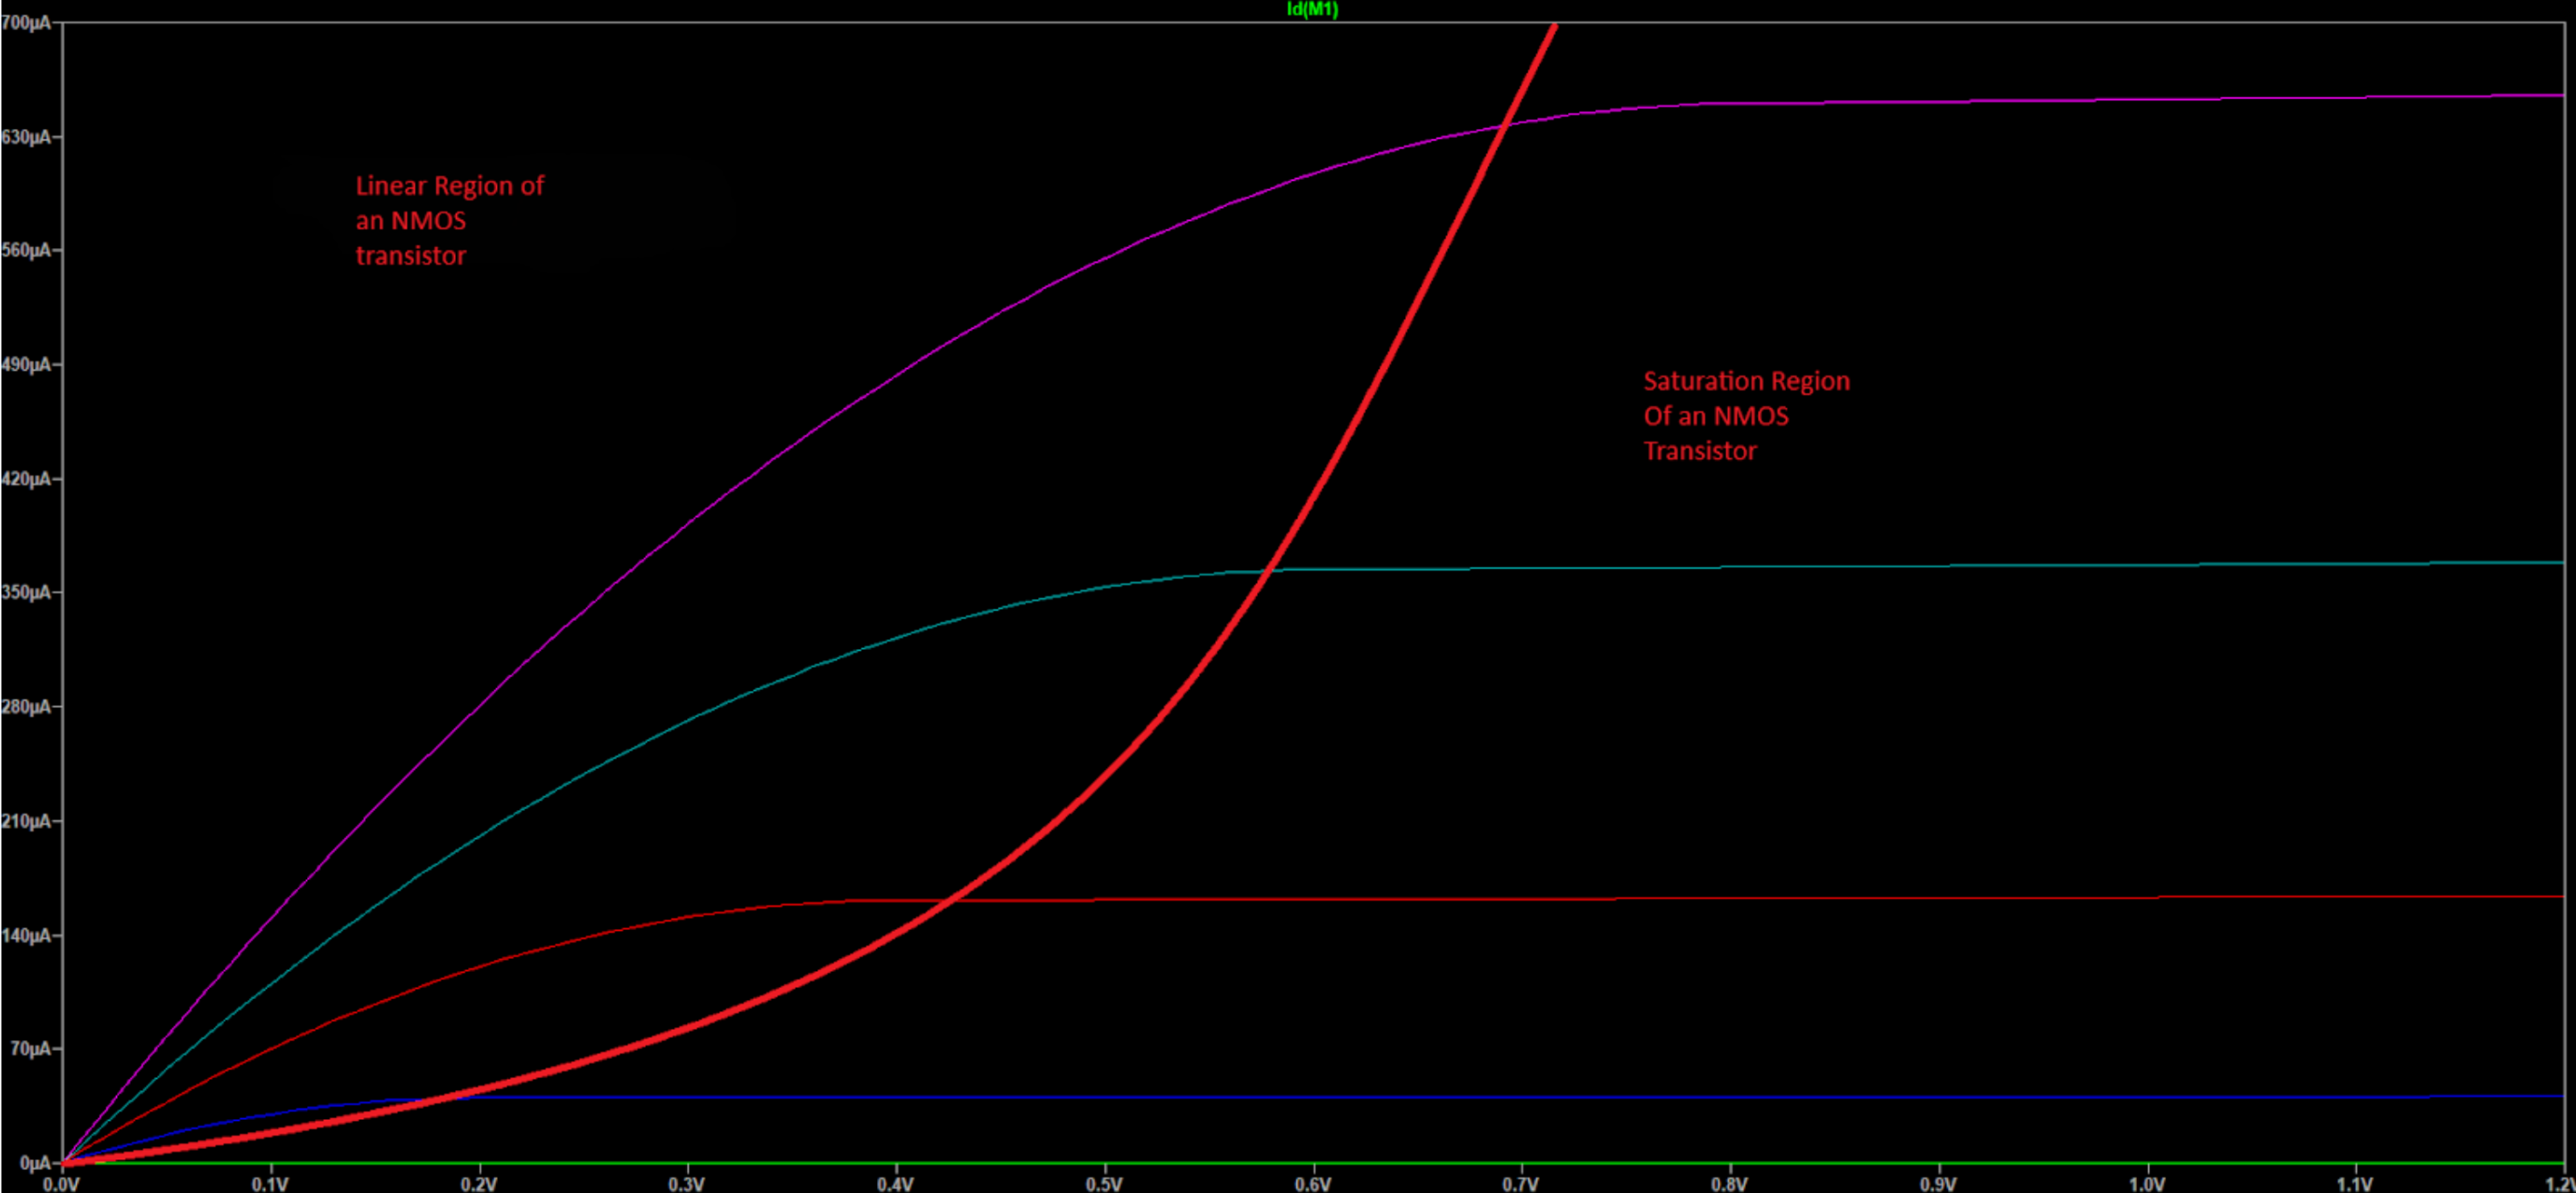
\includegraphics[width=0.8\textwidth]{NMOSSweep.png}
    \caption{NMOS I-V Characteristics showing Linear and Saturation regions for different $V_{GS}$ values.}
    \label{fig:nmos_sweep}
\end{figure}

\subsubsection*{Linear Region}
This occurs when:

\begin{equation}
V_{DS} < V_{GS} - V_T
\end{equation}

In this region, the transistor behaves like a voltage-controlled resistor. The drain current is given by \textit{Equation 11}:

\begin{equation}
I_D = \beta \left[ (V_{GS} - V_T)V_{DS} - \frac{1}{2}V_{DS}^2 \right]
\end{equation}

where, if we refer to \textit{Equation 10} again:

\[
\beta = \frac{W}{L} \mu_n C_{ox} = \frac{W}{L} K_P
\]

Initially, the current $I_D$ increases approximately linearly with $V_{DS}$.

\subsubsection*{Saturation Region}
This occurs when:

\begin{equation}
    V_{DS} \geq V_{GS} - V_T
\end{equation}

In this region, the channel is \emph{pinched off} near the drain, and the drain current becomes almost independent of $V_{DS}$:

\begin{equation}
    I_D = \frac{\beta}{2}(V_{GS} - V_T)^2(1 + \lambda V_{DS})
\end{equation}

The slight upward slope in the $I_D$--$V_{DS}$ characteristics is due to \textbf{channel-length modulation}, represented by the parameter $\lambda$ (typically $\lambda = 0.02$).
Parameters have been defined below and in the Background section. \textit{Listing 1} shows the code used to generate the graph (next page).

\newpage

\begin{lstlisting}[caption=NMOS Sweep Simulation Code, label=lst:nmos_sweep]
* Task 1 Extended: Sweep VDS and VGS (multiple curves)
* nmos_DC_sweep.cir is a netlist.

* Sets the VGS value to 1.2V (can be changed to sweep different values)
.param VGSVAL=1.2 

* Tells us the voltages that we will use and the connections (so V_GS is a DC source and it has a gate connection (0V DC), same with the Drain)
VGS G 0 DC {VGSVAL}
VDS D 0 DC 0
* Tells us the transistor dimensions (gate width (W), channel length (L)) along with source and body voltage.
M1 D G 0 0 NLEVEL1 W=10u L=1u

.model NLEVEL1 NMOS LEVEL=1 VTO=0.4 KP=200u LAMBDA=0.02
* VTO is V_th, KP = transconductance parameter, LAMBDA is the channel-length modulation factor.

.dc VDS 0 1.2 0.01 VGS 0.4 1.2 0.2
* plots the drain current (I(M1)s) against VDS for different VGS values from 0.4V to 1.2V in steps of 0.2V
.plot DC I(M1)s 
.end

* Comments start with asterisk
* First line is title (can be anything)
* Last line must be .END (or .end as SPICE is case insensitive)
* Node names: numbers or alphanumeric
* Node 0 is always ground
* Component values: scientific notation (1e-12) or units (1p, 1n, 1u, 1m, 1k, 1meg)
\end{lstlisting}

\subsubsection*{Parameter Definitions}
\begin{itemize}
    \item $I_D$ : Drain current
    \item $V_{GS}$ : Gate-to-source voltage
    \item $V_T$ : Threshold voltage
    \item $V_{DS}$ : Drain-to-source voltage
    \item $\mu_n$ : Electron mobility
    \item $C_{ox}$ : Oxide capacitance per unit area
    \item $W$ : Channel width
    \item $L$ : Channel length
    \item $\beta = \dfrac{W}{L}\mu_n C_{ox}$ : Process transconductance parameter
    \item $\lambda$ : Channel-length modulation parameter (typically $\lambda = 0.02$)
\end{itemize}

\subsection{PMOS I-V Characteristics (Second Task - Lab 1 Part 1)}

We can see the PMOS Sweep for a few specified $V_{SG}$ values in \textit{Figure 3}. The explanation of the code will be shown below:

\begin{figure}
    \centering
    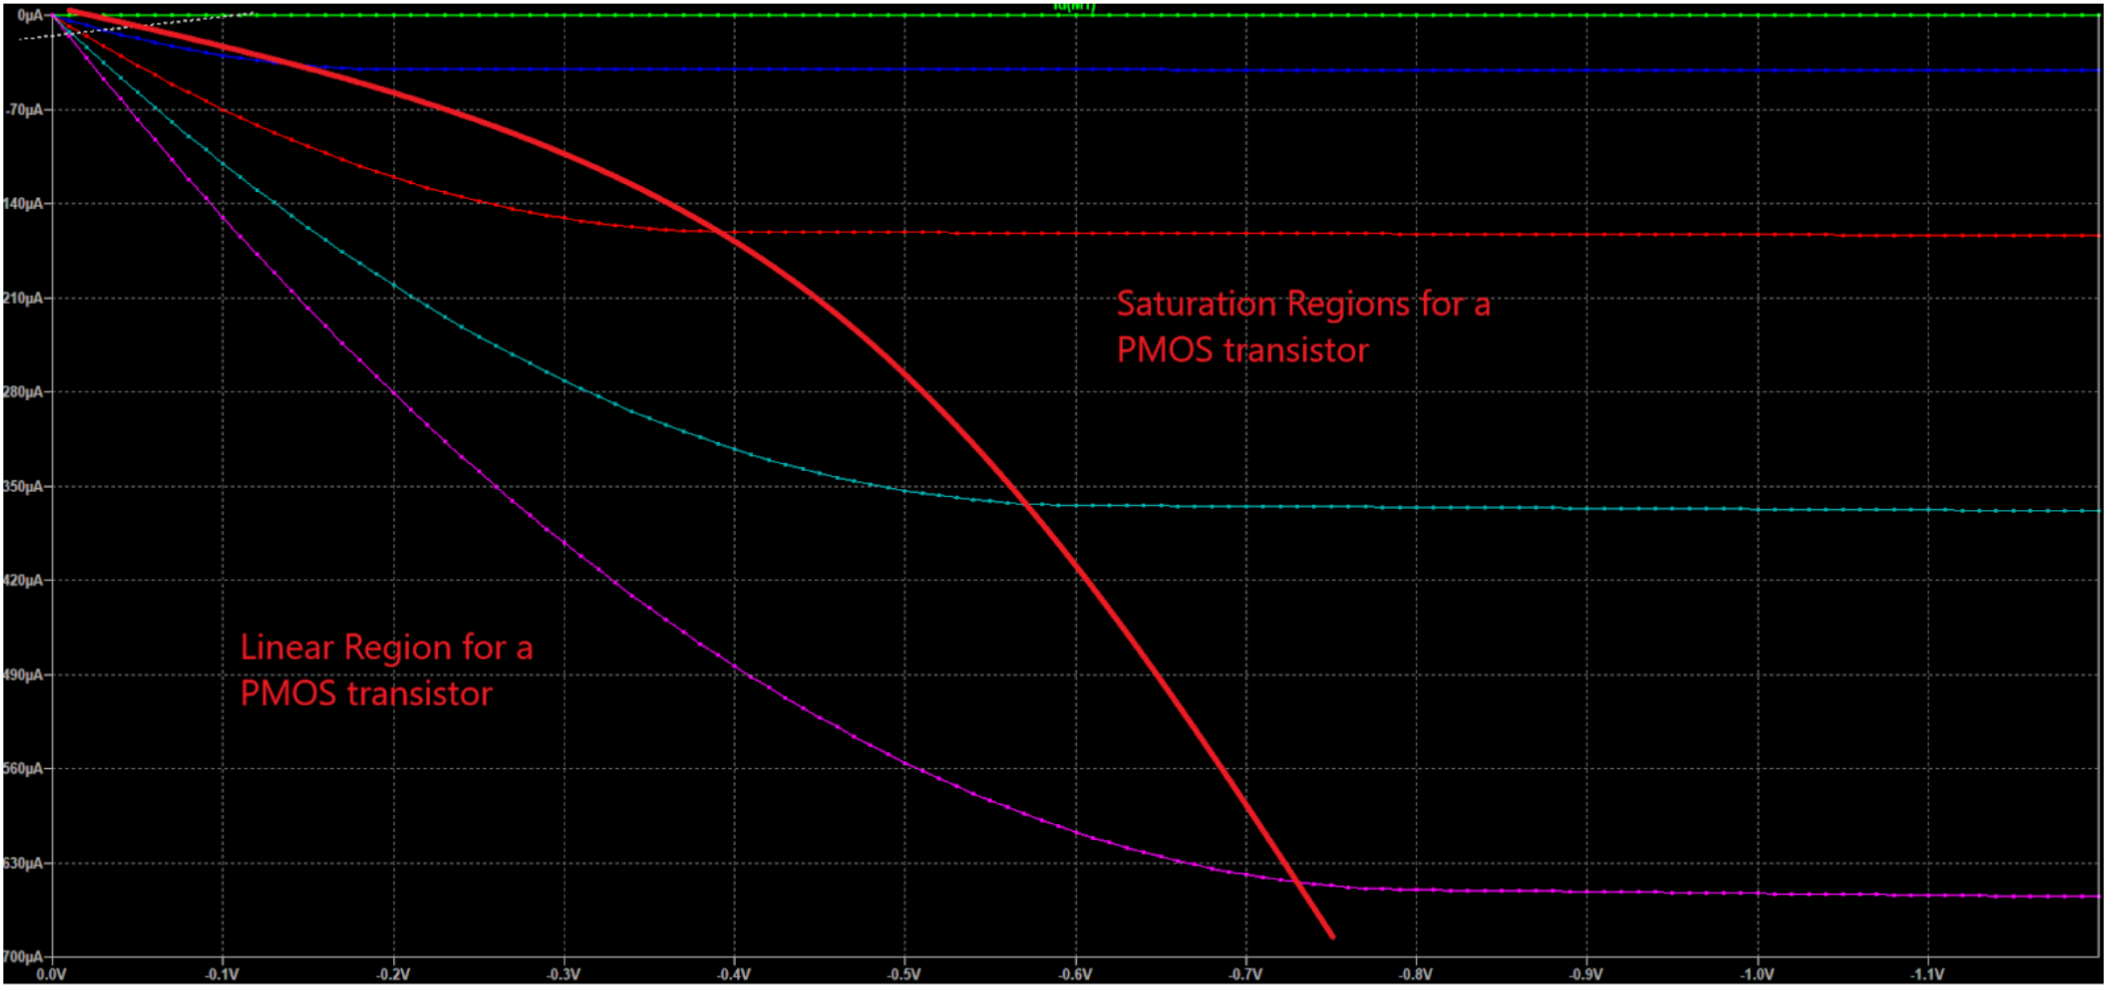
\includegraphics[width=0.8\textwidth]{PMOSSweep.png}
    \caption{PMOS I-V Characteristics showing Linear and Saturation regions for different $V_{SG}$ values.}
    \label{fig:pmos_sweep}
\end{figure}

For a PMOS transistor, all voltages are \textbf{negative} relative to the NMOS device. The key differences are:

\begin{itemize}
    \item $V_{SG}$ (source-to-gate voltage) replaces $V_{GS}$
    \item $V_{SD}$ (source-to-drain voltage) replaces $V_{DS}$
    \item The drain current $I_D$ flows from the \textbf{source to the drain}, opposite to that of the NMOS
\end{itemize}

\subsection*{Linear Region}
This occurs when:
\[
V_{SD} < V_{SG} - |V_T|
\]
The transistor behaves like a voltage-controlled resistor. The drain current is given by:
\[
I_D = \beta \left[ (V_{SG} - |V_T|)V_{SD} - \frac{1}{2}V_{SD}^2 \right]
\]
where:
\[
\beta = \frac{W}{L}\mu_p C_{ox} = \frac{W}{L} K_P
\]
Initially, $I_D$ increases approximately linearly with $V_{SD}$.

\subsection*{Saturation Region}
This occurs when:
\[
V_{SD} \geq V_{SG} - |V_T|
\]
In this region, the channel is \emph{pinched off} near the drain, and the current becomes almost independent of $V_{SD}$:
\[
I_D = \frac{\beta}{2}(V_{SG} - |V_T|)^2(1 + \lambda V_{SD})
\]
The small increase in $I_D$ with $V_{SD}$ is due to \textbf{channel-length modulation}, represented by $\lambda$.

\subsection*{Calculation with Example Values from PMOS Sweep}
For a PMOS transistor with:
\[
V_{SG} = 1.2~\text{V}, \quad |V_T| = 0.4~\text{V}
\]
the boundary between the linear and saturation regions occurs at:
\[
V_{SD} = V_{SG} - |V_T| = 1.2 - 0.4 = 0.8~\text{V}
\]
On an $I_D$--$V_{DS}$ plot, this corresponds to:
\[
V_{DS} = -0.8~\text{V}
\]

indicating the same boundary but with reversed voltage polarity compared to NMOS operation.

For \( V_{GS} = -1.2\,\text{V} \):

\[
\text{Saturation occurs when } V_{DS} \le -0.8\,\text{V}
\]
\[
\text{Linear region: } -0.8\,\text{V} < V_{DS} < 0\,\text{V}
\]
\[
\text{Saturation region: } V_{DS} \le -0.8\,\text{V}
\]

\[
\text{Linear Region } (V_{SD} < V_{SG} - |V_T|):
\]
\[
I_D = -\beta\left[(V_{SG} - |V_T|)V_{SD} - \tfrac{1}{2}V_{SD}^2\right]
\]

\[
\text{Note: Current is negative (flows from source to drain)}
\]

\[
\text{Example calculation for } V_{SG} = 1.2\,\text{V}, \; V_{SD} = 0.4\,\text{V}:
\]
\[
\beta = \frac{W}{L} \cdot K_P = \frac{10}{1} \cdot 200\,\mu = 2\,\text{mA/V}^2
\]
\[
I_D = -2\,\text{mA/V}^2 \times \left[(1.2 - 0.4)\times0.4 - 0.5\times0.4^2\right]
\]
\[
I_D = -2\,\text{mA/V}^2 \times [0.32 - 0.08]
\]
\[
I_D = -2\,\text{mA/V}^2 \times 0.24
\]
\[
I_D = -0.48\,\text{mA} = -480\,\mu\text{A}
\]

\[
\text{Saturation Region } (V_{SD} \ge V_{SG} - |V_T|):
\]
\[
I_D = -\frac{\beta}{2}(V_{SG} - |V_T|)^2(1 + \lambda V_{SD})
\]

\[
\text{Example for } V_{SG} = 1.2\,\text{V}, \; V_{SD} = 1.2\,\text{V}:
\]
\[
I_D = -\left(\frac{2\,\text{mA/V}^2}{2}\right) (0.8)^2 (1.024)
\]
\[
I_D = -1\,\text{mA/V}^2 \times 0.64 \times 1.024
\]
\[
I_D = -0.655\,\text{mA} = -655\,\mu\text{A}
\]

Current is negative (opposite polarity to NMOS) and the curves mirror NMOS behavior, with saturation boundaries at $V_{DS} = -(V_{SG} - |V_T|)$.
This is shown in \textit{Figure 3}.

\newpage

\begin{lstlisting}[caption=PMOS Sweep Simulation Code, label=lst:pmos_sweep]
* TASK 2: PMOS I-V DC Sweep with Multiple VSG Curves

* Define gate-source voltage as parameter (negative for PMOS)
.param VGSVAL=-1.2

* Gate voltage source: negative voltage for PMOS operation
* Connected between gate (G) and ground (0)
VGS G 0 DC {VGSVAL}

* Drain voltage source: starts at 0V, swept negative
VDS D 0 DC 0

* PMOS transistor M1:
* Connections: Drain=D, Gate=G, Source=0(GND), Bulk=0(GND)
* In normal PMOS, bulk connects to highest potential (VDD)
* Here, 0V used  as reference for ease of simulation, refer to source in report.
* Geometry: Width=10um (same as NMOS), Length=1um
M1 D G 0 0 PLEVEL1 W=10u L=1u

* Level 1 PMOS model parameters:
* VTO   = -0.4V   : Threshold voltage (negative for PMOS)
* KP    = 200uA/V^2: Transconductance (typically half of NMOS in reality)
* LAMBDA= 0.02V^-1: Channel-length modulation (same as NMOS)
.model PLEVEL1 PMOS LEVEL=1 VTO=-0.4 KP=200u LAMBDA=0.02

* DC Sweep Analysis:
* Primary sweep: VDS from 0V to -1.2V in -0.01V steps (negative direction)
* Secondary sweep: VGS from -0.4V to -1.2V in -0.2V steps
* This generates 5 curves (VGS = -0.4, -0.6, -0.8, -1.0, -1.2V)
.dc VDS 0 -1.2 -0.01 VGS -0.4 -1.2 -0.2

* Plot drain current (will be negative for PMOS)
.plot DC I(M1)

* End of netlist
.end
\end{lstlisting}

\subsection{Beta Sweep}

\subsubsection{Question 1: Identification}

\begin{itemize}
    \item VGS = 1.2V (from .param VGSVAL=1.2)
    \item VDS = 1.2V (from .param VDSVAL=1.2)
    \item L = 1um (from M1 line: L=1u)
\end{itemize}

\subsubsection{Question 2A\: Model Parameter Definitions}

\textbf{VTO (Threshold Voltage):}
Symbol: $V_T$ or $V_{th}$. Units: Volts (V).

Zero-bias threshold voltage - the minimum gate-source voltage required to form a conducting inversion channel. Below this voltage, the transistor is in cutoff. Determined by gate material work function, oxide thickness, substrate doping, and interface charges. In our simulation: VTO = 0.4V (NMOS), -0.4V (PMOS).

\textbf{KP (Transconductance Parameter):}
Symbol: $k'$ or $\mu C_{ox}$. Units: A/V$^2$.

Intrinsic transconductance parameter representing the product of carrier mobility ($\mu$) and gate oxide capacitance per unit area ($C_{ox}$):
\begin{equation}
KP = \mu \cdot C_{ox} = \mu \cdot \frac{\varepsilon_{ox}}{t_{ox}}
\end{equation}

Determines current drive capability. The gain factor is $\beta = (W/L) \cdot KP$, so $I_D \propto KP$. NMOS typically has 2-3$\times$ higher KP than PMOS due to higher electron mobility. In our simulation: KP = 200$\mu$A/V$^2$ for both types.

\textbf{LAMBDA (Channel-Length Modulation):}
Symbol: $\lambda$. Units: V$^{-1}$. Default: 0.0.

Channel-length modulation coefficient accounting for effective channel shortening as $V_{DS}$ increases in saturation. Without LAMBDA, saturation curves would be perfectly flat (infinite output resistance). With LAMBDA:
\begin{equation}
I_D(sat) = \frac{\beta}{2}(V_{GS} - V_T)^2(1 + \lambda V_{DS})
\end{equation}

Output resistance: $r_o = 1/(\lambda I_D)$. Inversely proportional to channel length: $\lambda \propto 1/L$. Analogous to inverse Early voltage in BJTs. In our simulation: $\lambda = 0.02$ V$^{-1}$, causing $\sim$2.4\% current increase across 1.2V $V_{DS}$ range.


\subsubsection{Question 2B\: Model Assumptions}

The standard textbook equation for saturation current is:
\begin{equation}
I_D = \frac{\beta}{2}(V_{GS} - V_T)^2 \quad \text{where } \beta = \frac{W}{L} \cdot \mu_n C_{ox}
\end{equation}

The complete SPICE Level 1 equation is:
\begin{equation}
I_D = \frac{KP}{2} \cdot \frac{W_{eff}}{L_{eff}} \cdot (V_{GS} - VTO)^2 \cdot (1 + LAMBDA \cdot V_{DS})
\end{equation}

To simplify the SPICE model to match textbook equations, the following assumptions are made:

\textbf{1. LAMBDA = 0 (or very small):}
The term $(1 + \lambda V_{DS})$ is set to 1, neglecting channel-length modulation. This assumes perfectly flat I-V curves in saturation with infinite output resistance. In our simulation, $\lambda = 0.02$ causes only a $\sim$2.4\% variation, which is small but non-zero.

\textbf{2. No body effect ($\gamma = 0$ or $V_{SB} = 0$):}
The body effect modifies threshold voltage as:
\begin{equation}
V_T = V_{T0} + \gamma(\sqrt{|2\phi_F + V_{SB}|} - \sqrt{|2\phi_F|})
\end{equation}
When bulk and source are both at ground ($V_{SB} = 0$), this term vanishes and $V_T = V_{T0}$, which is our case.

\textbf{3. Long-channel approximation:}
Velocity saturation is neglected, assuming drift velocity remains proportional to electric field. Valid for $L \geq 1\mu$m. Short-channel effects (DIBL, threshold roll-off) are ignored.

\textbf{4. No mobility degradation:}
Carrier mobility $\mu$ is assumed constant, independent of $V_{GS}$. In reality, high vertical electric fields reduce mobility, but Level 1 ignores this.

\textbf{5. Ideal effective dimensions:}
$W_{eff} = W$ and $L_{eff} = L$ (no parasitic effects). When $LD = WD = XL = XW = DEL = 0$, drawn and effective dimensions are equal.

\textbf{6. Subthreshold conduction ignored:}
For $V_{GS} < V_T$, Level 1 assumes $I_D = 0$. In reality, exponential subthreshold current exists: $I_D \propto \exp(V_{GS}/nV_t)$.

\textbf{Verification of equivalence:}
If $KP = \mu_n C_{ox}$, then:
\begin{equation}
\beta_{textbook} = \frac{W}{L} \cdot \mu_n C_{ox} = \frac{W}{L} \cdot KP = \beta_{SPICE}
\end{equation}
With $LAMBDA = 0$, $V_{SB} = 0$, and ideal geometry, the equations become identical.

\subsubsection{Simulation Verification}

\textbf{VTO verification:} DC sweep shows $I_D \approx 0$ at $V_{GS} = 0.4$V, confirming threshold. Current increases dramatically for $V_{GS} > 0.4$V.

\textbf{KP verification:} From beta\_w\_sweep.cir:
\begin{equation}
\frac{dI_D}{dW} = 65.54~\mu\text{A}/\mu\text{m (measured)} = \frac{KP}{2L}(V_{GS}-VTO)^2(1+\lambda V_{DS}) = 65.54~\mu\text{A}/\mu\text{m (theory)}
\end{equation}
Perfect agreement validates KP = 200~$\mu$A/V$^2$.

\textbf{LAMBDA verification:} In saturation at $V_{GS} = 1.2$V:
\begin{itemize}
    \item $V_{DS} = 0.8$V: $I_D = 642~\mu$A, $(1+0.02\times0.8) = 1.016$ → +1.6\%
    \item $V_{DS} = 1.2$V: $I_D = 656~\mu$A, $(1+0.02\times1.2) = 1.024$ → +2.4\%
\end{itemize}

Measured current increase: $(656-642)/642 = 2.2\%$ $\approx 2.4\%$ predicted. Slight upward slope in saturation curves confirms $\lambda = 0.02$V$^{-1}$.

\textbf{Body effect assumption:} $V_{SB} = 0$ throughout (source and bulk both grounded), so $V_T = VTO = 0.4$V constant. Confirmed by consistent threshold across all simulations.

\textbf{Subthreshold assumption:} Setting $V_{GS} = 0.3$V $< V_T$ yields $I_D \approx 0$ as Level 1 predicts, though real devices show exponential subthreshold current ($\sim$pA range).

\subsection{How Does SPICE Work?}

SPICE is the circuit simulator that we have been using so far. It models electronic circuits by solving nonlinear differential-algebraic equations derived from Kirchhoff’s laws. The general form of the circuit equations is:
\begin{equation}
\mathbf{f}(\mathbf{x}, \dot{\mathbf{x}}, t) = 0
\end{equation}
where \(\mathbf{x}\) represents the vector of unknown node voltages and branch currents.

Using modified nodal analysis (MNA), SPICE forms equations of the type:
\begin{equation}
\mathbf{C} \, \dot{\mathbf{v}} + \mathbf{G}(\mathbf{v}) = \mathbf{i}_s(t)
\end{equation}
where:
- \(\mathbf{C}\) is the capacitance matrix,  
- \(\mathbf{G}(\mathbf{v})\) represents nonlinear conductances (resistors, diodes, transistors, etc.),  
- \(\mathbf{i}_s(t)\) represents source currents.

For transient analysis, SPICE discretizes the time derivative using a numerical integration method such as Backward Euler [source]:
\[
\dot{\mathbf{v}}(t_n) \approx \frac{\mathbf{v}_n - \mathbf{v}_{n-1}}{\Delta t}
\]
This transforms the equations into a system of nonlinear algebraic equations:
\begin{equation}
\mathbf{F}(\mathbf{v}_n) = \mathbf{G}(\mathbf{v}_n) + \frac{\mathbf{C}}{\Delta t} (\mathbf{v}_n - \mathbf{v}_{n-1}) - \mathbf{i}_s(t_n) = 0
\end{equation}

To solve this system, SPICE uses the \textbf{Newton–Raphson method}, an iterative root-finding algorithm for nonlinear equations. Given a function \(\mathbf{F}(\mathbf{v})\), the goal is to find \(\mathbf{v}\) such that:
\begin{equation}
\mathbf{F}(\mathbf{v}) = 0
\end{equation}
Starting from an initial guess \(\mathbf{v}^{(0)}\), the method iteratively refines the estimate using:
\[
\mathbf{J}(\mathbf{v}^{(k)}) \, \Delta \mathbf{v}^{(k)} = -\mathbf{F}(\mathbf{v}^{(k)}), \quad
\mathbf{v}^{(k+1)} = \mathbf{v}^{(k)} + \Delta \mathbf{v}^{(k)}
\]

Here is a simple worked example of the Newton-Raphson method:

We want to solve the nonlinear equation
\begin{equation}
f(x) = x^2 - 2 = 0
\end{equation}
whose root is \(\sqrt{2}\).

The Newton–Raphson iteration formula is:
\[
x_{n+1} = x_n - \frac{f(x_n)}{f'(x_n)}
\]

For our function \(f(x) = x^2 - 2\),
\[
f'(x) = 2x
\]
so the iteration becomes:
\[
x_{n+1} = x_n - \frac{x_n^2 - 2}{2x_n}
\]

Let the initial guess be \(x_0 = 1\). Then:
\[
x_1 = 1 - \frac{1^2 - 2}{2(1)} = 1.5
\]
\[
x_2 = 1.5 - \frac{1.5^2 - 2}{2(1.5)} = 1.4167
\]
\[
x_3 = 1.4167 - \frac{1.4167^2 - 2}{2(1.4167)} = 1.4142
\]

After three iterations, \(x_3 \approx 1.4142\), which is very close to the true value of \(\sqrt{2}\).

Here, \(\mathbf{J}(\mathbf{v})\) is the \textbf{Jacobian matrix} of \(\mathbf{F}\), defined as:
\begin{equation}
\mathbf{J}(\mathbf{v}) =
\begin{bmatrix}
\frac{\partial F_1}{\partial v_1} & \frac{\partial F_1}{\partial v_2} & \cdots & \frac{\partial F_1}{\partial v_n} \\
\frac{\partial F_2}{\partial v_1} & \frac{\partial F_2}{\partial v_2} & \cdots & \frac{\partial F_2}{\partial v_n} \\
\vdots & \vdots & \ddots & \vdots \\
\frac{\partial F_n}{\partial v_1} & \frac{\partial F_n}{\partial v_2} & \cdots & \frac{\partial F_n}{\partial v_n}
\end{bmatrix}
\end{equation}
The Jacobian represents how each equation in \(\mathbf{F}\) changes with respect to each variable in \(\mathbf{v}\). In circuit terms, it corresponds to the small-signal conductance matrix, which describes the local linear behavior of the nonlinear circuit.

The Newton–Raphson method repeats this process until the solution converges, meaning:
\begin{equation}
\|\Delta \mathbf{v}^{(k)}\| < \epsilon
\end{equation}
for some small tolerance \(\epsilon\).

In summary:
1. SPICE forms nonlinear equations via modified nodal analysis.  
2. It discretizes time derivatives for transient analysis.  
3. It applies the Newton–Raphson method to iteratively solve the nonlinear system.  
4. The Jacobian matrix captures how circuit equations respond to voltage and current changes, enabling efficient convergence to the correct solution.


\section{Report Checklist}

\begin{itemize}
    \item Lab 1 Part 1
    \item N-Type characteristics
    \item P-Type characteristics
    \item MOSFET operation
    \item Parts that constitute a MOSFET and what altering them does to the operation of the MOSFET.
    \item Explanation of the PMOS and NMOS operation regions.
    \item What measurements were taken and how they were taken.
    \item Explanation of the graphs plotted and what they signify.
    \item Include code snippets of the simulation code used.
    \item Include graphs plotted.
    \item Analysis of the results.
    \begin{enumerate}
        \item DC Analysis of NMOS and PMOS and explanation of what DC analysis is.
        \item Task 1: NMOS DC I-V sweep with annotations.
        \item Task 2: PMOS DC I-V sweep with annotations.
        \item Gain factor calculation and explanation.
        \item Beta explanation with Python example.
        \item Task 4 Iterative solution
    \end{enumerate}
    \item Lab 1 Part 2
    \item Explain what static analysis is.
    \item Draw an annotated schematic of the inverter circuit.
    \item Explain the operation of the inverter circuit.
    \item 1B, Annotate the file (All 7 lines)
    \item TASK 1C: DC Modes You have simulated the DC transfer characteristic of a CMOS inverter by sweeping the input voltage Vin from 0 V to 5 V. Plot the 
    output voltage Vout against Vin. On your plot of Vout vs. Vin, clearly mark and label the following five operating points:
    A: Vin=0, B: Vin=1, C: Vin=2.5, D: Vin=4, E: Vin=5, For each point (A–E), identify the operating region of both the NMOS and PMOS transistors: Cutoff
    Triode (Linear) or Saturation, showing it as a table, and approximate Vout at each point.
    \item TASK 1D, NMOS pull up example, show the sweep as well, then answer these 5 questions:
    \item Q1. (1 mark) What is the highest output voltage reached in the NMOS pull-up version? Why does it not reach 5 V?
    \item Q2. (1 mark) Explain what happens to the NMOS pull-up transistor when Vin=0. Is it conducting?
    \item Q3. (1 mark) Describe what would happen if this NMOS-only inverter drove another CMOS logic gate. What are the risks?
    \item Q4. (1 mark) Why does a PMOS transistor avoid this issue? How does it behave differently from NMOS in pull-up?
    \item Q5. (2 marks) On your NMOS-only inverter plot, annotate the output voltage limit and mark the region where a 1 cannot be produced.
    \item TASK 2: TASK 2: CMOS Inverter Design for Delay Specification
    Use LTspice and theoretical models to design an inverter that meets timing specifications. Analyze
    performance using simulation and transistor-level delay theory (including propagation delay, rise/fall
    time, capacitive loading).
    \item TASK 2 Question 1 Transient Simulation and Analysis.
    \item TASK 2 Question 2 RC Delay Model.
    \item TASK 2 Question 3 Design and New Alternatives for performance.
    \item TASK 2 Question 4 Selection of questions to be answered.
\end{itemize}

\end{document}